\chapter{Introduction and Related Work}
Before answering the question, this chapter will set out to examine the topic of flow and look at what it means.

The frontrunner behind \textit{flow} is Mihaly Csikszentmihalyi, an Hungarian professor of psychology who's work includes studies of hapiness and creativity. He describes flow as an optimal experience, where one is in a state of control and balance: \textit{"When the information that keeps coming into awareness is congruent with goals, psychic energy flows effortlessly."} \citep{flow} He describes an optimal experience as \textit{"[s]ituations in which attention can be freely invested to achieve a person's goals, because there is no disorder to straighten out, no threat for the self to defend against."} \citep{flow} Flow is very much connected to challenge and skills. It can be compared to the challenge of climbing a mountain: each time a rock climber overcomes a great challenge, he is left as a more capable and skilful person \citep{flow}. While climbing the mountain, he is in a state of flow --- there is a perfect balance of what he is capable of and what is demanded of him. In other words, the difficulty of climbing the mountain fits the climber, so that it is neither too easy nor too hard. Figure \ref{fig:flowModel} shows the \textit{flow model}, which is often used when designing videogames. One should be challenged enough to not become bored. Likewise, the challenge cannot be too great compared to one's skill sets, since this will result in anxiety. In practice, one would fluctuate between these two states, but only touching them tangentially.

\begin{figure}[htbp]
\centering
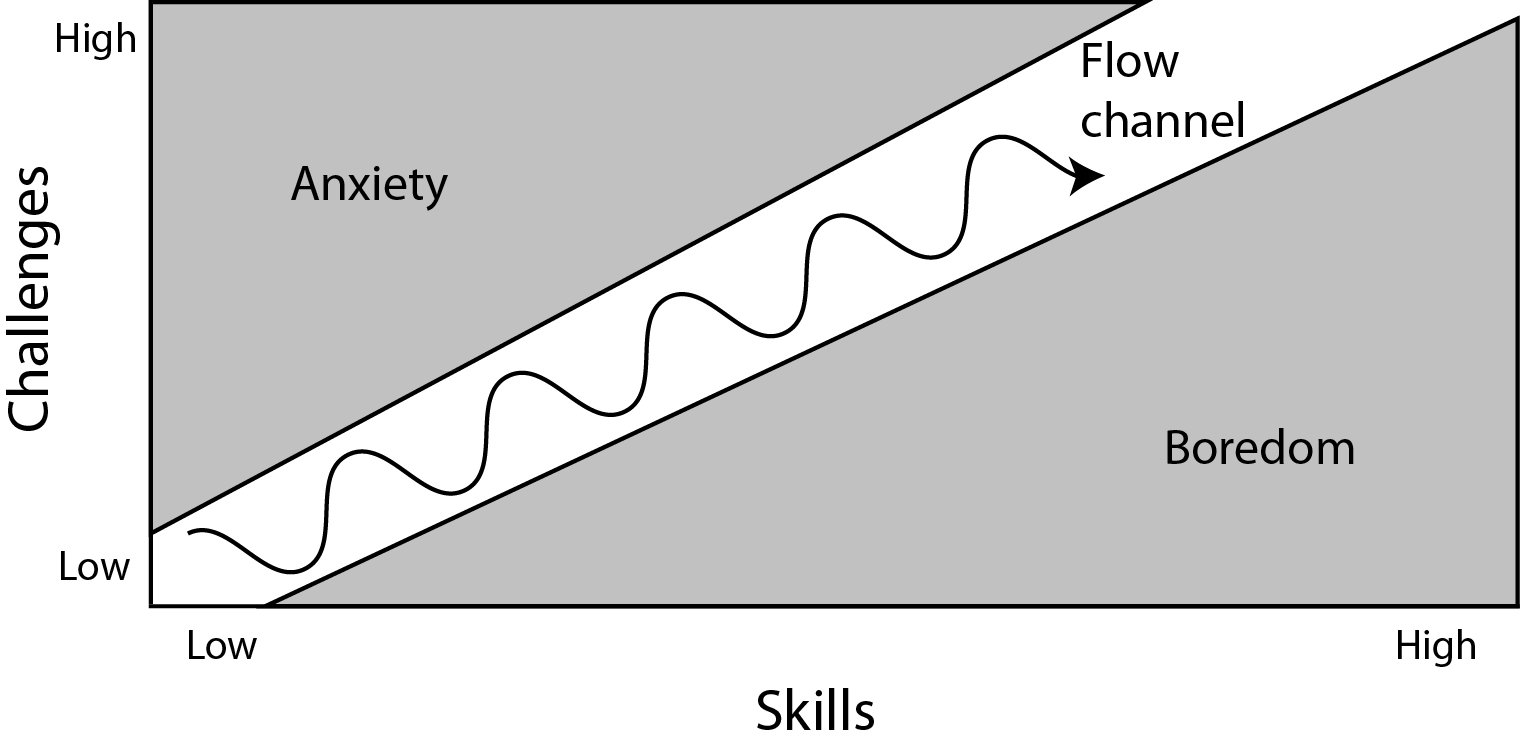
\includegraphics[width=0.70\textwidth]{Pictures/flow_model}
\caption{The flow state can be described as a balance between difficulty and skill \citep{artOfGameDesign}.}
\label{fig:flowModel}
\end{figure}

\cite{flow} has found that people report extreme joy, sometimes described as "a feeling of ecstasy", in many different types of contexts. What has been found to be a common element of all those cases is activities that are goal-directed and bounded by rules. They were challenging activities that could not be done without the appropriate skills \citep{flow}. Additionally, they were situations with clear and immediate feedback, say, a tennis match or a game of chess. With each action, it is clear whether or not one gets closer to accomplish one's goal(s). Furthermore, the experience of enjoying the flow state often occurs in activities outside ordinary life, e.g. games and sports. Flow has been described as \textit{"[l]acking the sense of worry about losing control that is typical in many situations of normal life."} \citep{flow}. It's a sensation where one' often loses self-consciousness and the sense of time and place.

One key element in experiencing flow is that the activity has an end in itself. This is described as an \textit{autotelic experience}, which means that doing something is an reward in itself. In other words, an activity should be intrinsically rewarding, where one doesn't expect external rewards such as money or recognition by peers. Many things in life yield extrinsic rewards, i.e., we perform activities because we \textit{have} to, not because we \textit{want} to (e.g., having a boring day-job in order to earn money to live).

To summarize, \cite{flowTwo} describe two main conditions for entering the flow state: \textit{perceived challenges that stretch, but don't overmatch, existing skills} and \textit{clear goals coupled with immediate feedback about the progress being made}. Furthermore, flow is a subjective state that has the following characteristics:

\begin{itemize}
\item intense and focused concentration on the present moment
\item merging of action and awareness
\item loss of reflective self-consciousness (i.e., loss of awareness of oneself as a social actor)
\item a sense that one can control one's actions; that is, a sense that one can in principle deal with the situation because one knows how to respond to whatever happens next
\item distortion of temporal experience (typically, a sense that time has passed faster than normal)
\item experience of the activity as intrinsically rewarding, such that often the end goal is just an excuse for the process
\end{itemize}